\documentclass{article}

\usepackage[utf8]{inputenc}
\usepackage[T1]{fontenc}
\usepackage{amsmath}
\usepackage{amsfonts}
\usepackage{amssymb}
\usepackage[version=4]{mhchem}
\usepackage{stmaryrd}
\usepackage{bbold}
\usepackage{graphicx}
\usepackage{adjustbox}
\usepackage{tocloft}   % For TOC formatting
\usepackage{geometry}  % For margins
\usepackage{titlesec}  % For section formatting
\usepackage{fancyhdr}
\usepackage{float}
\usepackage[stable]{footmisc}
\usepackage{hyperref}  % For clickable links in TOC (load last)
\usepackage{mdframed}  
\usepackage{listings}  
\usepackage{subcaption}
\input{style.tex}


% Document styling
\geometry{margin=1in}

% Customize section formatting (option 2: let titlesec handle the label)
\titleformat{\section}
  {\normalfont\Large\bfseries} % format
  {\thesection}                % label
  {0.5em}                      % separation
  {\rule{\textwidth}{0.4pt}\vspace{0.5em}\newline} % before-code

% adding a header
\pagestyle{fancy}
\fancyhf{}
\lhead{Problem Set 5}
\rhead{Henrik Berger - Romain Fernex}
\cfoot{ \thepage}
\renewcommand{\headrulewidth}{0.8pt}

\title{Problem Set 5 - Macroeconomics}
\author{Henrik Berger - Romain Fernex}
\date{February 2025}

\begin{document}

\maketitle
\tableofcontents
\newpage

\section{Literature review}

\begin{figure}[H]
    \centering
    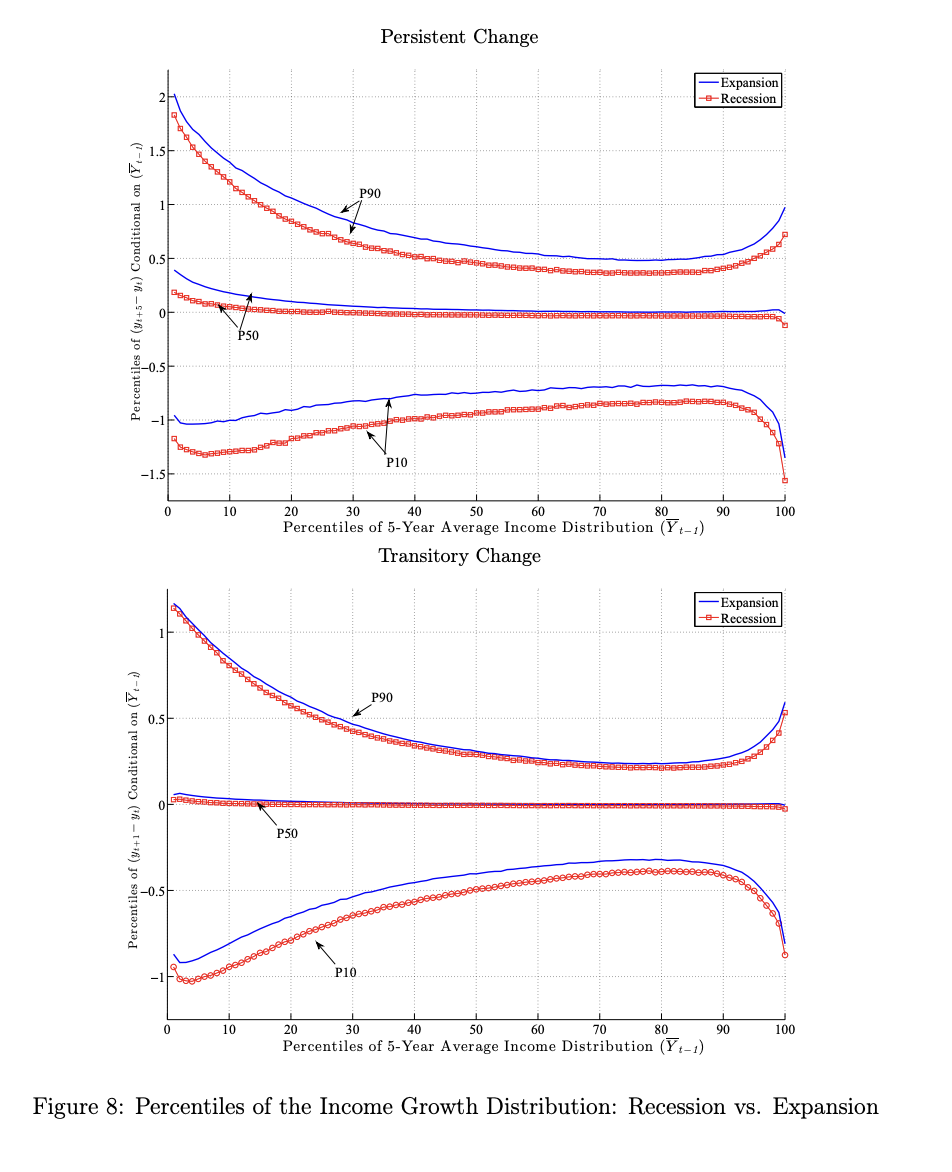
\includegraphics[width=0.8\textwidth]{figures/Screenshot 2025-11-20 at 6.16.10 AM.png}
\end{figure}

Figure 8 shows that recessions reshape the distribution of income growth by pushing both upper and lower percentiles downward, with a much stronger shift in the lower tail. For both 5-year and 1-year changes, workers with low past average income face the widest forward-looking ranges (P90 near 1.8 and P10 near –1.4), while those in the upper-middle of the distribution face the narrowest bands before risk rises again for top earners. In recessions, the P90 curve moves down by roughly 10 to 15 log points across almost all income groups, but the P10 falls by even more, often 15 to 20 log points, while the median barely changes. This creates a clear downward tilt in the shock distribution: large upward movements become much less likely, and large losses become more likely. The authors emphasize that this pattern, visible for both persistent and transitory shocks, reflects an increase in downside individual risk rather than a broad rise in volatility. It also appears consistently across the income distribution despite large underlying differences in baseline risk. This makes the macro mechanism unambiguous: aggregate downturns transmit risk primarily through sharper exposure to severe income losses, rather than through a general widening of outcomes, concentrating the burden of recessions in the lower tail of individual earnings changes.

\section{Exercise I}

\subsection*{1)}
The program solved by any agent $i$ is as follows : 
$$\begin{aligned}
    \max_{c^i_t,l^i_t}&\sum_{t=0}^{\infty}\beta^t(u(c^i_t)-l^i_t)\\
    \text{s.t} \quad &c^i_t+a^i_t = l^i_twe^i_t+(1+r)a^i_t+(1-e^i_t)\delta\\
    &a^i_{t+1}\geq \bar{a}>\frac{-\delta }{r}
\end{aligned}$$
Let's write the Bellman equations for each type : 
\begin{itemize}
    \item Employed agent (e) : 
    $$\begin{aligned}
        &V^e(a) = \max _{a',l} u(lw+(1+r)a-a')-l+\alpha V^e(a')+(1-\alpha) V^u(a')\\
        &\text{s.t} \quad a'\geq \bar{a}
    \end{aligned}$$
    \item Unemployed agent (u) : 
    $$\begin{aligned}
        &V^e(a) = \max _{a',l} u(\delta +(1+r)a-a')+(1-\rho) V^e(a')+\rho V^u(a')\\
        &\text{s.t} \quad a'\geq \bar{a}
    \end{aligned}$$
\end{itemize}

\subsection*{2)}
\textbf{A) Employed agent}
\begin{enumerate}
    \item We derive the FOCs in a' and l : We denote $\mu_e\ge0$ the shadow value of the borrowing constraint for the employed 
    $$\begin{aligned}
        \left\{\begin{aligned}
            &u'(c) = \beta [\alpha (V^e)'(a') + (1-\alpha)(V^u)'(a')]+\mu_e\quad (\text{in $a'$)}\\
            &wu'(c)=1 \quad  (\text{in $l$)}
        \end{aligned} \right. 
    \end{aligned}$$
    \item We derive the Envelope condition in a : using the FOC in l 
    $$(V^e)'(a)=(1+r)u'(c)=\frac{1+r}{w}$$
    \item We iterate over a : w and r are exogenous and time-invariant
    $$(V^e)' (a')=\frac{1+r}{w}$$
\end{enumerate}
\textbf{B) Unemployed agent}
\begin{enumerate}
    \item  We derive the FOCs in a' : We denote $\mu_u\ge0$ the shadow value of the borrowing constraint for the employed c
    $$u'(c) = \beta [(1-\rho)(V^e)'(a')+\rho(V^u)'(a')]+\mu_u$$
    \item We derive the Envelope condition in a : 
    $$(V^u)'(a)=(1+r)u'(c)$$
    \item Iterate over a : 
    $$(V^u)'(a') = (1+r)u'(c')$$
\end{enumerate}
\textbf{C) Euler Equations}
\begin{itemize}
    \item Employed Agent : 
    $$u'(c) \geq  \beta[\alpha\frac{(1+r)}{w}+(1-\alpha)(1+r)u'(c')]=\beta (1+r)[\frac{\alpha}{w}+(1-\alpha)u'(c')]$$
    \item Unemployed Agent : 
    $$u'(c) \geq \beta (1+r)[\frac{1-\rho}{w}+\rho u'(c')]$$
\end{itemize}

\subsection*{3)}
Let's assume the credit constraint binds for the unemployed and that $\bar{a}=0$ (no borrowings). Let's denote $a_u$ the savings of the unemployed and $a_e$ the savings of the employed. Since constraint binds we have $a_u=0$. First, using the credit constraint equations we can find the two possible consumption levels for the unemployed agent : 
$$\begin{aligned}
    &c_{uu}=\delta +(1+r)a_u = \delta \\
    &c_{eu}=\delta +(1+r)a_e
\end{aligned}$$
Now, for the employed agents, consumptions is pinned down by the labor supply tradeoff equation which does not vary based on one's previous state. Thus we always have the following consumption level for employed agents : for the sake of simplicity we normalize the wage to 1 for this equation and all the results to come 
$$c_e = (u')^{-1}(\frac{1}{w})=(u')^{-1}(1)$$

\subsection*{4)}
The employed agent is borrowing constrained if $\mu_e >0$ (constraint is binding)  and $a_e = 0$ : Assuming the unemployed are constrained as in 3), this gives us the following condition
$$\begin{aligned}
    u'(c_e)&>\beta (1+r)[\alpha +(1-\alpha)u'(c_{eu})]\\
    1&> \beta (1+r)[\alpha + (1-\alpha)u'(\delta +(1+r)a_e)]\\
    \frac{1}{\beta(1+r)}&>\alpha+(1-\alpha)u'(\delta +(1+r)a_e)
\end{aligned}$$

\subsection*{5)}
By the same logic, the unemployed agent is borrowing constraint if $\mu_u >0$ and $a_u=0$:
$$\begin{aligned}
    &\left\{\begin{aligned}
    u'(c_{uu}) > \beta (1+r)[(1-\rho)+\rho u'(c_{uu})]\\
    u'(c_{eu})> \beta (1+r)[(1-\rho)+\rho u'(c_{uu})]
    \end{aligned}\right.\\
    \Leftrightarrow &\left\{\begin{aligned}
    &u'(\delta ) > \beta (1+r)[(1-\rho)+\rho u'(\delta)]\\
    &u'(\delta +(1+r)a_e)> \beta (1+r)[(1-\rho)+\rho u'(\delta)]
    \end{aligned}\right.
\end{aligned}
$$
Since $\delta < \delta +(1+r)a_e$ and since $u$ is concave, we have that $u'(\delta) >u'(\delta +(1+r)a_e)$ so satisfying the second condition is sufficient by itself (since it implies that the first one is satisfied as well)

\subsection*{6)}
Let's determine the savings of the employed : from q2 we have 
$$\left\{\begin{aligned}
    u'(c) \geq \beta (1+r)(\frac{\alpha}{w}+(1-\alpha)u'(c'))\\
    u'(c) = 1
\end{aligned} \right.$$
Assuming the employed is unconstrained $\mu_e=0$ and $a_e>0$ we have : 
$$1=\beta (1+r)(\alpha +(1-\alpha)u'(c_{eu}))$$
Then, using q3 we get : 
$$1=\beta (1+r)[\alpha +(1-\alpha)u'(\delta +(1+r)a_e)]$$
Let's rearrange the terms to get $a_e$ :
$$a_e = [(u')^{-1}(\frac{1}{1-\alpha}[\frac{1}{\beta(1+r)}-\alpha])-\delta]\frac{1}{1+r}$$
Labor supply is a static choice and disutility of labor is linear, so the labor-supply first-order condition fixes the marginal utility of consumption at $u'(c_e)=1/w$
This pins down employed consumption uniquely, regardless of past asset holdings or unemployment history.
Intertemporal smoothing is then absorbed entirely by savings $a_e$, not by consumption.

\subsection*{7)}
We have : we have a unit mass of agent so $n=1$\\
\textbf{A) number of employed}
$$\begin{aligned}n_e &= n_{ee}+n_{ue}\\
& = \alpha n_e + (1-\rho)n_u \\
&= \alpha n_e + (1-\rho)(1-n_e)
\end{aligned}$$
Thus we get : 
$$n_e = \frac{1-\rho}{2-\alpha-\rho}$$
\textbf{B) number of employed who became unemployed}
$$n_{eu}= (1-\alpha)n_e= \frac{(1-\alpha)(1-\rho)}{2-\alpha-\rho}$$
\textbf{C) number of people who stayed unemployed}
$$n_{uu}=1-n_e-n_{eu}=\frac{\rho(1-\alpha)}{2-\alpha-\rho}$$
Then we have : since n is normalized to 1
$$\begin{aligned}
    \text{unemployment rate } = n_u = n_{eu}+n_{uu}= \frac{1-\alpha}{2-\alpha -\rho}\\
    \text{employment rate}= n_e = \frac{1-\rho}{2-\alpha-\rho}
\end{aligned}$$

\subsection*{8)}
Assuming the unemployed are borrowing constrained and the employed are not, we use the results from q6 and q7 to get :
$$A = n_ea_e+n_ua_u=\frac{1-\rho}{2-\alpha-\rho}[(u')^{-1}(\underbrace{\frac{1}{1-\alpha}[\frac{1}{\beta(1+r)}-\alpha]}_{\equiv B})-\delta]\frac{1}{1+r}$$

\subsection*{9)}
Let's derive $A$ with respect to $\alpha$ and investigate the sign of this derivative : 
$$\frac{dA}{d\alpha}=a_e\times  \frac{dn_e}{d\alpha } + n_e \times \frac{da_e}{d\alpha }$$
It's easy to see that $\frac{dn_e}{d\alpha }$ is postive since the number of employed increases as the probability of staying employed goes up. Let's compute $\frac{da_e}{d\alpha }$ and pin down its sign : 
$$\begin{aligned}
    \frac{dB}{d\alpha }(u'')^{-1}(B) &= [\frac{1}{(1-\alpha)^2}(\frac{1}{\beta (1+r)}-\alpha)-\frac{1}{1-\alpha}](u'')^{-1}(B)\\
    &= [\frac{1}{(1-\alpha)^2}(\frac{1}{\beta(1+r)}-1)](u'')^{-1}(B)
\end{aligned}$$
We classically assume that $1+r >\frac{1}{\beta}$ thus the left most term is positive and the whole derivative is negative since $u''<0$ (concavity). 
Thus we have an ambiguity : when $\alpha $ goes up the number of people employed goes up, so more people save, BUT the amoung of savings per person goes down. 
$$\frac{dA}{d\alpha}=\underbrace{a_e\times  \frac{dn_e}{d\alpha }}_{>0} + \underbrace{n_e \times \frac{da_e}{d\alpha }}_{<0}$$



\section{Exercise II}

\subsection{Model Description}

\subsubsection*{State and Control Variables}
\begin{itemize}
    \item 3 state variables : 
    \begin{enumerate}
        \item assets\footnote{what was saved at the last period} $a$ : continuous 
        \item productivity $w_j(s)$ (high $|$ low) : binary ($s_L$,$s_H$) and following a markov process, two different value grids
        \item employment status $j$ (employed $|$ self employed) : binary ("e","se")
    \end{enumerate}
    \item 3 choice variables : 
    \begin{enumerate}
        \item savings $a'$ 
        \item employment status $j'$ 
        \item labour $l$ : continuous, only relevant to the self-employed as the wage-employed does not have the option to adjust his workload (comprised in wage contract)
    \end{enumerate}
\end{itemize}

\subsubsection*{Exogenous Parameters}
\begin{itemize}
    \item $\bar{l}$ labour supplied under wage-contract (fixed)
    \item $r\in [0,1]$ the interest rate on savings 
    \item $b>0$ unemployment benefits 
\end{itemize}

\begin{simplebox}{On Productivity}
Two separate value grids (wage-employed $|$ self-employed) : with $y^H_{se} > y^H_{e}>0$
\begin{itemize}
    \item self-employed : $w_{se}(s_L)=0$ (low productivity state) $|$ $w_{se}(s_H)=y^H_{se}$ (high productivity state)
    \item wage-employed : $w_{e}(s_L) = b$ (low productivity state) $|$ $w_{e}(s_H)=y^H_{e}$ (high productivity state)
\end{itemize}
\end{simplebox}

\subsubsection*{Functional Assumptions}
\begin{itemize}
    \item The disutility of work is assumed to be a weighted isoelastic function of labor supply (increasing, convex) : with $\psi$ the weight of labor disutility, $\gamma$ the inverse of the Frisch elasticity of labor supply.
    $$\phi(l)=\psi \frac{l^{1+\gamma}}{1+\gamma}$$
    \item The utility of consumption is assumed to follow a standard CRRA functional form 
    $$u(c) = \frac{c^{1-\mu}-1}{1-\mu}$$
\end{itemize}

\subsubsection*{Optimization Programms}
\textbf{Employed}
$$\begin{aligned} &V_e(a,s)=\max_{a',j'}u(c)-\bar{l}+E[\beta V_{j'}(a',s')]\\
&\text{s.t}\quad 
    c+a'=(1+r)a+\phi(\bar{l})\times w_{e}(s) \quad \text{if }j'=e \\
    &\qquad c+a'=(1+r)a+\phi(\bar{l})\times w_{e}(s)-F \quad \text{if }j'=se\\
&\qquad a' \geq 0
\end{aligned}$$

\noindent \textbf{Self-Employed}
$$\begin{aligned} &V_{se}(a,s)=\max_{a',j',l}u(c)-l+E[\beta V_{j'}(a',s')]\\
&\text{s.t}\quad c+a'=(1+r)a+\phi(l)\times w_{se}(s) \quad \forall j'\in \{e,se\} \\
&\qquad a' \geq 0
\end{aligned}$$

\subsection{Coding Challenges}
There were three core difficulties we had to face when coding the VFI : 
\begin{enumerate}
    \item We enable the agent to pick the optimization programm he will face in the next period, conditional on the constraints he his facing currently. This means we had to consider two separate value functions at the same time and keep in mind that they have to interact with one another. 
    \item The high number of control variables swiftly inflates the size of the arrays we have to manipulate to get the policy and value functions. This forced us to carefully look at the dimensions of each element to avoid multiplication errors. 
    \item The fact that there is not a perfect overlap between the variables that the employed and the self-employed optimize over made things fairly confusing at first although it ended up being less messy than we had feared in the final version of the code. 
\end{enumerate}

\subsection{Model Results}
\subsubsection*{Optimal saving decision}
% Asset policy function
\begin{figure}[H]
    \centering
    % First Image
    \begin{subfigure}[b]{0.45\textwidth}
        \centering
        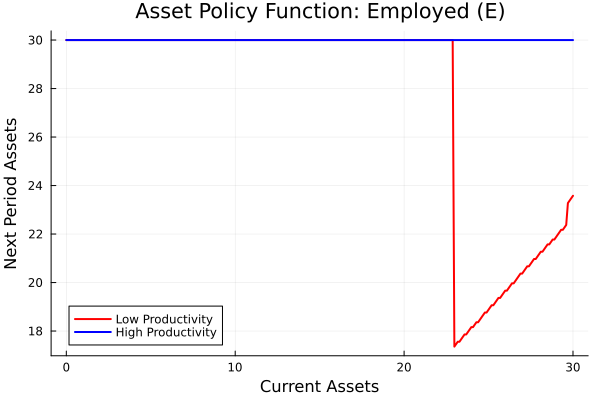
\includegraphics[width=\textwidth]{figures/asset_policy_employed_1.png}
        \caption{When currently wage-employed}
    \end{subfigure}
    \hfill % Adds flexible space between the images
    % Second Image
    \begin{subfigure}[b]{0.45\textwidth}
        \centering
        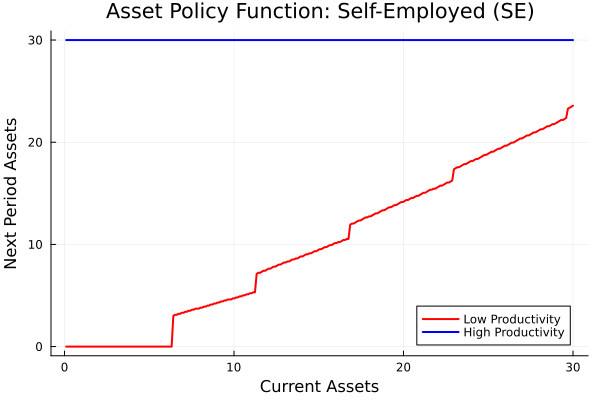
\includegraphics[width=\textwidth]{figures/asset_policy_self_employed_1.png}
         \caption{When currently self-employed}
    \end{subfigure}
    \caption{Next period assets as a function of current assets}
\end{figure}
\begin{simplebox}{Proposition n°1}
    An agent that is currently employed and has low productivity saves as much as possible until he can afford to liquidate some of his assets to start his own business. 
\end{simplebox}

\noindent \textbf{Mechanism : } When the agent starts with a low amount of assets he prefers to save as much as possible of his work income in order to ensure he won't forever remain below the wealth threshold (here $a = 23$ + labor income from wage-job) that would enable him to pay the cost of setting up his own business in the future. Then, once current assets exceed the threshold, he uses some of them, as well as his labor income, to pay for the cost of going self-employed, which gives him the opportunity to reduce his workload, maximizing his utility.  

\subsubsection*{Optimal employment decision}
% Employment decision
\begin{figure}[H]
    \centering
    % First Image
    \begin{subfigure}[b]{0.45\textwidth}
        \centering
        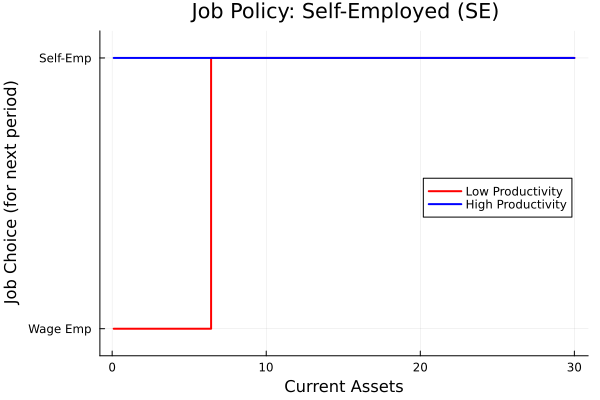
\includegraphics[width=\textwidth]{figures/job_policy_self_employed_1.png}
        \caption{High persistence + Low revenue gap}
    \end{subfigure}
    \hfill % Adds flexible space between the images
    % Second Image
    \begin{subfigure}[b]{0.45\textwidth}
        \centering
        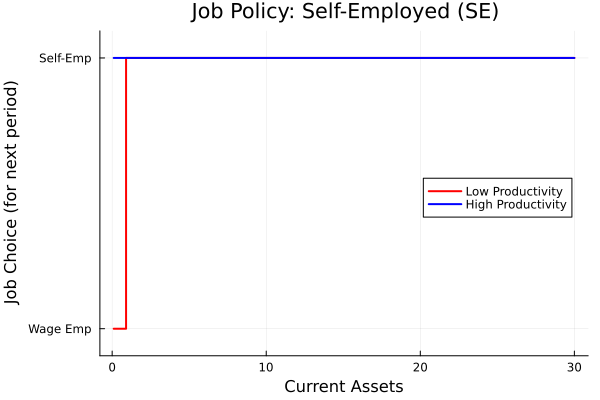
\includegraphics[width=\textwidth]{figures/job_policy_self_employed_3.png}
         \caption{Moderate persistence +  Large revenue gap}
    \end{subfigure}
    \caption{Next period employment status as a function of current assets}
\end{figure}
\begin{simplebox}{Proposition n°2}
    When the high productivity state is more likely and  yields more for the self-employed, even the poor self-employed currently in the bad state prefers to keep his business running. 
\end{simplebox}

\noindent \textbf{Mechanism :} In the above example we use two different parameter combinations :
\begin{itemize}
    \item set-up 1) where the gap between high productivity state payoffs is low and where transitions from a state to the opposite one are rare 
    \item set-up 2) where the gap between high productivity state payoffs is high and where transitions from a state to the opposite one are thrice as frequent. 
\end{itemize}
In the latter case, the expected gains of remaining self-employed are significantly higher so he prefers to keep his business open instead of going back to wage employment. In the former, however, expected gains when starting in the bad state are much lower which pushes the poor entrepreneur to seek a more stable form of employment until he can reach the wealth threshold enabling him to earn back his independence. 

\subsection{Limitations}
A salient issue with this model is that self-employed agents consistently exploit labor flexibility to work fewer hours than wage employees. We believe this 'lazy entrepreneur' outcome arises because the marginal disutility of labor rises faster than the marginal benefit of additional income (consumption smoothing).\\
A potential remedy could be to introduce wealth directly in the utility function (as in Saez et al, 2018). If agents derive utility directly from holding wealth, they would have an incentive to work hard to accumulate assets even when their consumption needs are essentially satisfied.

\subsection{IMPORTANT : Running the code}
\begin{enumerate}
    \item Download the two julia scripts from moodle (uploaded as .txt files)
    \item Convert both files back to .jl  and put them in the same directory
    \item Modify the export/import directory named root-path in the main file to
    \item Run ONLY the main file : as we propose two different parameter set-ups, the program asks you which one you want to run at the beginning 
\end{enumerate}

\section{Reference}
Fatih Guvenen, Serdar Ozkan, and Jae Song, The Nature of Countercyclical Income Risk, Journal of Political Economy 2014 122:3, 621-660\\
Pascal Michaillat \& Emmanuel Saez, 2018. "A New Keynesian Model with Wealth in the Utility Function," 2018 Meeting Papers 1276, Society for Economic Dynamics.

\end{document}


